  
\SSbreak\\
\emph{Source: One Hundred Problems - 4th Edition Q93}\\
\emph{Proposer: \Phobo}\\
\emph{Problem ID: 106}\\
\emph{Date: 2021-01-21}\\
\SSbreak

\SSpsetQ{

    After paying Joe what is due, the PSC team find themselves at the gates of a destitute underground research facility. Upon exploring the ransacked and decaying tomb they find themselves in a laboratory experimenting with teleportation. The PSC try to get it working:\\

    .19, Brainy, and Yuchan enter the teleporter where they are each positioned randomly along a 1m strip.\\
    
     For the teleporter to work, .19 and Brainy must be less than half a meter apart, and .19 and Yuchan must also be less than half a meter apart. \\
    
    If the probability that the teleporter works is $\frac mn$, find $100m +n$

}\bigskip

\begin{solution}[Solution by \Phobo]\hfil\medskip

    The problem statement can be reduced to this: \\

    Let \(a,b\) and \(c\) be real numbers randomly chosen from the interval $[0,1]$, if the probability of $|a-b|<\frac{1}{2}$ and $|b-c| <\frac{1}{2}$ can be expressed as $\frac{m}{n}$, find $100m+n$.\\


    I will pursue a geometrical approach using a 3D space with coordinates (a,b,c), such that for every triplet (a,b,c) there exist one and only point enclosed in the cube whose vertices are (0,0,0) (1,0,0) (1,1,0) (0,1,1) and so on. The probability we are seeking can be seen as ratio between volumes, in particular the volume of the intersection of the two solids $|a-b|<\frac{1}{2}$ and $|b-c| <\frac{1}{2}$, over the volume of the cube with side 1. Let's focus on finding what the solid $|a-b|<\frac{1}{2}$ looks like: if we consider the plane c=0, with some trivial analytic algebra we can draw the following polygon:
    \begin{figure}[ht]
        \centering
    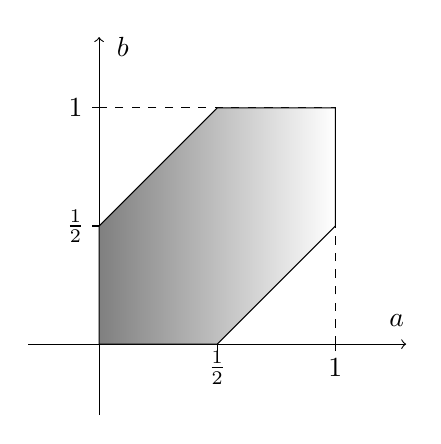
\begin{tikzpicture}[scale=3]
    \draw[->] (-0.3,0) -- (1.3,0) node at (1.26,0.1) {$a$};
    \draw[->] (0,-0.3) -- (0,1.3) node at (0.1,1.26) {$b$};;
    \draw (1,-0.03) -- (1,0.03);
    \draw (-0.03,1) -- (0.03,1);
    \draw (0.5,-0.03) -- (0.5,0.03);
    \draw (-0.03,0.5) -- (0.03,0.5);
    \draw[dashed] (1,0) -- (1,1) -- (0,1);
    \node at (1,-0.1) {$1$};
    \node at (-0.1,1) {$1$};
    \node at (0.5,-0.1) {$\frac{1}{2}$};
    \node at (-0.1,0.5) {$\frac{1}{2}$};
    \shadedraw[left color=gray,right color=white]  (0,0) -- (0.5,0) -- (1,0.5) -- (1,1) -- (0.5,1) -- (0,0.5) -- (0,0);
    \end{tikzpicture}
    \end{figure}
    Introducing the 3rd dimension, $|a-b|<\frac{1}{2}$ turns out to be an hexagonal prism (the base is shown above) whose height is 1 (along the c-axis). Similarly $|b-c| <\frac{1}{2}$ is the same solid, but rotated 90 degrees around the line parallel to the b-axis and going through the point($\frac{1}{2}$,$\frac{1}{2}$,$0$). Let's now compute the intersection between those solids, which turns out to be the sum of few smaller solids, in particular: 2 cubes with side $\frac{1}{2}$, 2 square pyramids with base length and height $\frac{1}{2}$ and 4 triangular prism, having height $\frac{1}{2}$ and an isosceles right triangle with side $\frac{1}{2}$ as base. Finally  the probability is $$\displaystyle p=\frac{2\cdot\frac{1}{8}+2\cdot\frac{1}{24}+4\cdot\frac{1}{8}}{1}=\frac{7}{12}$$ which leads to 712 as final answer.
\end{solution}\bigskip
